\documentclass{article}

\usepackage[backend=biber]{biblatex}
\addbibresource{metabolic.bib}

\usepackage{amsmath,amsfonts}

\usepackage{tikz}
\usetikzlibrary{matrix}

\title{Learning an integrated network of metabolites and proteins from knockout screens}

\author{Yuriy Sverchkov}

\begin{document}
\maketitle

\begin{abstract}
Learning an integrated network of metabolites and proteins from knockout (KO) screens.
Given knockout screens with large-scale MS measurements of protein, metabolite, and lipid abundances, as well as incomplete prior knowledge about
relevant regulatory, signaling, and metabolic pathways, we seek to elucidate the roles of uncharacterized actors and extend the network accordingly.
\end{abstract}

\section{Introduction}

\section{Background}

Prior related work includes:
\begin{itemize}
 \item \textcite{lee2008dynamic} present a flux-balance-analysis-based model that integrates signaling, metabolic, and regulatory networks.
\end{itemize}

Our approach is in some ways similar to nested effects model \parencite{citation-needed}.
A general effects model can be characterized by an effect matrix $F$ where columns correspond to knockouts and and the rows correspond to measured phenotypes or ``effects,'' and matrix entries correspond to differential expression.
The NEM factorizes $F = \Gamma \Theta$ where $\Gamma$ represents the propagation of a knockout to changes in gene activity among signaling genes (assumed to be the set of genes knocked out) and $\Theta$ represents the propagation of those changes to the measured effects.

\section{Method}

We may consider data available to us to come in one of a few possible forms:
\begin{enumerate}
 \item Quantitative measurements of particle abundances across conditions, including a wild-type (WT) condition.
 \item A binary call table of differential expression between each KO condition and the WT.
 \item A trinary ($-1, 0, +1$) call table of signed differential expression between each KO condition and the WT.
 \item A log-odds table that expresses the log-odds of differential expression.
\end{enumerate}

Similarly to the NEM, we consider a series of propagations of KO effects, expressed as matrices (which correspond to regulatory, signaling, and metabolic networks).

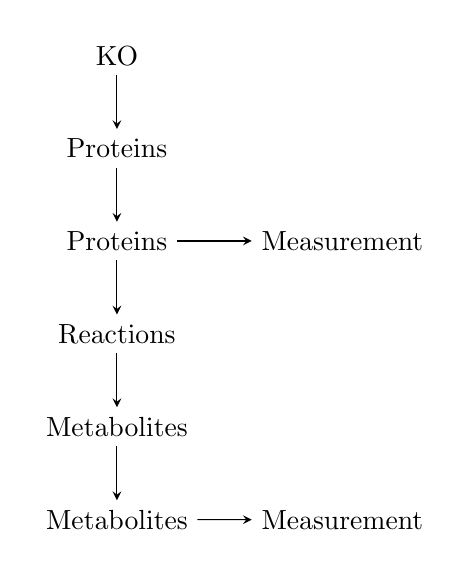
\begin{tikzpicture}
  \matrix (m) [matrix of nodes, row sep = 2em, column sep = 2em]
  {
    KO & \\
    Proteins & \\
    Proteins & Measurement \\
    Reactions & \\
    Metabolites & \\
    Metabolites & Measurement \\
  };
  \path[-stealth]
    (m-1-1) edge (m-2-1)
    (m-2-1) edge (m-3-1)
    (m-3-1) edge (m-3-2)
      edge (m-4-1)
    (m-4-1) edge (m-5-1)
    (m-5-1) edge (m-6-1)
    (m-6-1) edge (m-6-2);
\end{tikzpicture}

Question: where do lipids fit in?

\paragraph{Observation} if we can assume that there is no pathway for KOs to affect metabolites other than via its effect on proteins, could we treat the problem of predicting changes in metabolites given changes in proteins as a distinct problem from that of predicting changes in proteins given KOs?

\section{Results}

\section{Discussion}

\printbibliography

\end{document}